\documentclass{beamer}

\usepackage{cmap}
\usepackage[english,russian]{babel} % add eng,rus(base) package
\usepackage[T1,T2A]{fontenc}        % add eng,rus encoding support
\usepackage[utf8]{inputenc}         % add UTF8 support

% Use it for English document
%\usepackage[utf8]{inputenc} % add UTF8 support
%\usepackage{fontspec}       % to use any font known to the operating system
%\setmainfont{PT Serif}      % set defolt font

\usepackage{amsmath, amsfonts, amssymb, amsthm, mathtools} % add math support

\linespread{1}               % length between str
\setlength{\parindent}{16pt} % red str
\setlength{\parskip}{6pt}   % length between paragraphs

\usepackage[backend=biber, style=authoryear-icomp]{biblatex}
\addbibresource{$HOME/latex-templates/biblio.bib}            % path to bibliography base

\usetheme{Madrid}
\setbeamertemplate{frametitle}[default][center]

\renewcommand{\thefootnote}{\arabic{footnote}}
 % here is document's settings for russian


\title{Борис Ельцин}
\author{Немков Н.М.}
\institute[МГТУ]{МГТУ им. Н.Э. Баумана}
\date{06.05.2024}

\begin{document}

\begin{frame}
\maketitle
\end{frame}


%=============================== 1
\begin{frame}{}
	\begin{columns}
		\begin{column}{0.45\textwidth}

			12 июня 1991 был избран на должность президента РСФСР, после распада СССР его позиции как российского президента укрепились

		\end{column}


		\begin{column}{0.45\textwidth}

			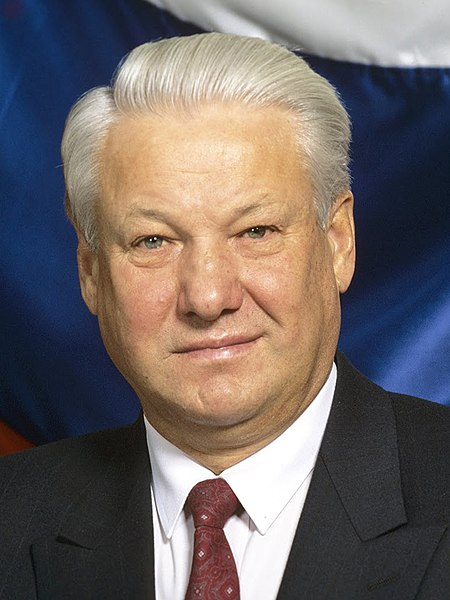
\includegraphics[width=1\textwidth]{images/elcin-1}

		\end{column}
	\end{columns}
\end{frame}

%================================ 2
\section{Внутренняя политика}
\begin{frame}{Внутреннаяя политика}

	Проводил курс по демократизации Политической системы

	Формировались конституционные основы политической системы

	В октябре 1993 года была принята конституция Российской Федерации

\end{frame}


%================================ 3
%================================ 4
\section{Внешняя политика}
\begin{frame}{Внешняя политика}

	1991-1996 -- неудачная попытка сближения с западом

	1996-1999 -- переорентация отношений преимущественно на Китай и индию

\end{frame}


%================================ 6
\section{Реформы}
\begin{frame}{Реформы}

	\textbf{Три кита}

	- Либерализация цен

	- Либерализация внешней торговли

	- Приватизация

\end{frame}


%================================ 7
\section{Итоги}
\begin{frame}{Итоги}

	Ни одна из реформ направленных на формирование конституционных основ политической системы России не ьыла пересмотрена и отменена

	Общий регресс агропромышленности

	Снижение престижа научного труда

	Наблюдался рост преступности
\end{frame}


\section{Благоданость}
\begin{frame}
	\centering
	\huge
	Спасибо за внимание!
\end{frame}


\end{document}
